%%%%%%%%%%%%%%%%%%%%%%%%%%%%%%%%%%%%%%%%%
% Beamer Presentation
% LaTeX Template
% Version 1.0 (10/11/12)
%
% This template has been downloaded from:
% http://www.LaTeXTemplates.com
%
% License:
% CC BY-NC-SA 3.0 (http://creativecommons.org/licenses/by-nc-sa/3.0/)
%
%%%%%%%%%%%%%%%%%%%%%%%%%%%%%%%%%%%%%%%%%

%----------------------------------------------------------------------------------------
%	PACKAGES AND THEMES
%----------------------------------------------------------------------------------------

\documentclass{beamer}

\usepackage[utf8x]{inputenc}
\usepackage[english,serbian]{babel}
\usepackage{pgfplots}
\pgfplotsset{compat=1.10}
\usetikzlibrary{calc} 

\definecolor{RYB1}{RGB}{128, 177, 211}
\definecolor{RYB2}{RGB}{251, 128, 114}
\definecolor{RYB3}{RGB}{253, 180, 98}


\mode<presentation> {

% The Beamer class comes with a number of default slide themes
% which change the colors and layouts of slides. Below this is a list
% of all the themes, uncomment each in turn to see what they look like.

%\usetheme{default}
%\usetheme{AnnArbor}
%\usetheme{Antibes}
%\usetheme{Bergen}
%\usetheme{Berkeley}
%\usetheme{Berlin}
%\usetheme{Boadilla}
%\usetheme{CambridgeUS}
%\usetheme{Copenhagen}
%\usetheme{Darmstadt}
%\usetheme{Dresden}
%\usetheme{Frankfurt}
%\usetheme{Goettingen}
%\usetheme{Hannover}
%\usetheme{Ilmenau}
%\usetheme{JuanLesPins}
%\usetheme{Luebeck}
\usetheme{Madrid}
%\usetheme{Malmoe}
%\usetheme{Marburg}
%\usetheme{Montpellier}
%\usetheme{PaloAlto}
%\usetheme{Pittsburgh}
%\usetheme{Rochester}
%\usetheme{Singapore}
%\usetheme{Szeged}
%\usetheme{Warsaw}

% As well as themes, the Beamer class has a number of color themes
% for any slide theme. Uncomment each of these in turn to see how it
% changes the colors of your current slide theme.

%\usecolortheme{albatross}
%\usecolortheme{beaver}
%\usecolortheme{beetle}
%\usecolortheme{crane}
%\usecolortheme{dolphin}
%\usecolortheme{dove}
%\usecolortheme{fly}
%\usecolortheme{lily}
%\usecolortheme{orchid}
%\usecolortheme{rose}
%\usecolortheme{seagull}
%\usecolortheme{seahorse}
%\usecolortheme{whale}
%\usecolortheme{wolverine}

%\setbeamertemplate{footline} % To remove the footer line in all slides uncomment this line
%\setbeamertemplate{footline}[page number] % To replace the footer line in all slides with a simple slide count uncomment this line

%\setbeamertemplate{navigation symbols}{} % To remove the navigation symbols from the bottom of all slides uncomment this line
}

\usepackage{graphicx} % Allows including images
\usepackage{booktabs} % Allows the use of \toprule, \midrule and \bottomrule in tables

%----------------------------------------------------------------------------------------
%	TITLE PAGE
%----------------------------------------------------------------------------------------

\title[Swift]{Swift - jezik budućnosti} % The short title appears at the bottom of every slide, the full title is only on the title page

\author[AD, PP, IM, IN]{Anđelković Dragica, Mandić Igor, Nikolić Igor, Petar Pejović} % Your name
\institute[Matf] % Your institution as it will appear on the bottom of every slide, may be shorthand to save space
{
Matematički fakultet \\ % Your institution for the title page
\medskip
\textit{andjelkovic.dragica96@gmail.com, igormandic996@gmail.com, \\ igor.nikolic032@hotmail.com, petar.pejovic8@gmail.com} % Your email address
}
\date{\today} % Date, can be changed to a custom date

\begin{document}

\begin{frame}
\titlepage % Print the title page as the first slide
\end{frame}

\begin{frame}
\frametitle{Uvod} % Table of contents slide, comment this block out to remove it
\tableofcontents % Throughout your presentation, if you choose to use \section{} and \subsection{} commands, these will automatically be printed on this slide as an overview of your presentation


%----------------------------------------------------------------------------------------
%	PRESENTATION SLIDES
%----------------------------------------------------------------------------------------

%------------------------------------------------


\end{frame}
%------------------------------------------------
\section{Nastanak i istorijski razvoj}
%------------------------------------------------
\begin{frame}
\frametitle{Nastanak i istorijski razvoj}
\begin{itemize}
\item  Razvoj je započeo 2010. godine Chris Lattner \cite{mastering_swift3}.
\item  Predstavljen je na međunarodnoj konferenciji programera 2014. godine, uz  Xcode 6 i OS 8 \cite{thenextweb_sajt}.
\item Apple je zvanično objavio Swift u decembru 2015. godine, kao projekat otvorenog k\^{o}da i pokrenuo je veb sajt.
\item Do danas je izbačeno 5 verzija Swift-a:
\begin{itemize}
\item{Swift 1.0} - 2014. godine
\item{Swift 2.0} - 2015. godine
\item{Swift 3.0} - 2016. godine
\item{Swift 4.0} - 2017. godine
\item{Swift 5.0} - 2019. godine
\end{itemize}
\end{itemize}

\end{frame}
%------------------------------------------------
\subsection{Mesto u razvojnom stablu}
%------------------------------------------------
\begin{frame}
\frametitle{ Mesto u razvojnom stablu}

\begin{figure}[h!]
\begin{center}
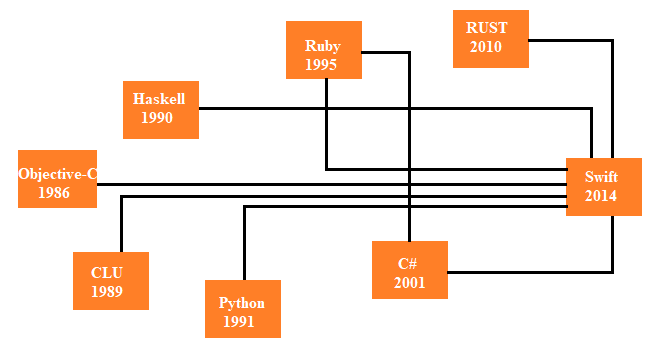
\includegraphics[scale=0.5]{razvojno_stablo.png}
\end{center}
\label{fig:razvojno_stablo}
\end{figure}

\end{frame}
%------------------------------------------------
\subsection{Uticaji drugih programskih jezika}
%------------------------------------------------
\begin{frame}
\frametitle{Uticaji drugih programskih jezika}
Preuzeti su određeni delovi iz različitih programskih jezika i poboljšani. Pregled preuzetih koncepata se nalaze u tabeli \ref{tab:koncepti}.

\begin{table}[h!]
\begin{center}
\caption{Preuzeti koncepti iz drugih programskih jezika}
\begin{tabular}{|l|l|} \hline
\label{tab:koncepti}
\textbf{Programski jezik} & \textbf{Preuzeti koncepti} \\ \hline
JavaScript & Struktura podataka - rečnik  \\ \hline
Scala i Opa & Zaključivanje tipova \\ \hline
Cold Fusion i JSP & Interpolacija Stringa \\ \hline
Python & Opciono naznačavanje kraja naredbe \\ \hline
Java i C\# & Protokoli (Interfejsi) \\ \hline
Lisp i Python & Torke (eng.~{\em Tuples}) \\ \hline
Lisp i JavaScript &  Closure funkcije \\ \hline
C\# i Objective-C & Označeni i neoznačeni celi brojevi \\ \hline
\end{tabular}
\end{center}
\end{table}
\end{frame}
%------------------------------------------------
\section{Osnovna namena, svrha i mogućnosti}
%------------------------------------------------
\begin{frame}
\frametitle{Osnovna namena, svrha i mogućnosti}
\begin{columns}[t]

\column{.5\textwidth}
Osnovna namena:
\begin{itemize}
\item iOS i macOS aplikacije
\item Aplikacije za iPhone i iPad uređaje
\item Server aplikacije
\item Razvoj IoT aplikacija
\item Za Linux operativni sistem
\item Radi se na
stvaranju Swift aplikacija koje će se izvršavati i na Android platformama.
\end{itemize}

\column{.5\textwidth} 
Neke od mogućnosti koje pruža \cite{mastering_swift3}:
\begin{itemize}
\item{Automatsko utvrđivanje tipova}
\item{Generički tipovi}
\item{Sintaksa zatvorenog izraza}
\item{Pseudoklase}
\item{Switch klase}
\item{Višestruki povratni tipovi}
\item{Preklapanje tipova}
\end{itemize}
Funkcija Xcode-a \textbf{Mix and match}.

\end{columns}
\end{frame}
%------------------------------------------------
\section{Osnovne osobine}
%------------------------------------------------
\begin{frame}
\frametitle{Osnovne osobine}
\begin{columns}[t] % The "c" option specifies centered vertical alignment while the "t" option is used for top vertical alignment

\column{.5\textwidth} % Left column and width
Osnovne osobine \cite{swift_programming} :
\begin{itemize}
\item{\textbf{Objektno orijentisan}}
\item{\textbf{Funkcionalan}}
\item{\textbf{Jasan}}
\item{\textbf{Bezbedan}}
\item{\textbf{Ekonomičan}}
\item{\textbf{Upravlja memorijom}}
\item{\textbf{Kompatibilnost sa razvojnim okruženjem Cocoa}}
\end{itemize}

\column{.5\textwidth} % Right column and width
Podržane paradigme:
\begin{itemize}
\item{\textbf{Objektno orijentisana paradigma}}
\item{\textbf{Funkcionalana paradigma}}
\item{\textbf{Imperativna paradigma}}
\end{itemize}

\end{columns}
\end{frame}
%------------------------------------------------

%------------------------------------------------
\begin{frame}
\frametitle{Osnovne osobine}
Zbog svojih osobina, 2016. godine, programski jezik Swift je bio najplaćeniji jezik u Americi. Na sledećem grafikonu (slika \ref{fig:grafikon}) prikazano je 10 najplaćenijih programskih jezika:

\begin{figure}[hbt!]
\begin{tikzpicture}
\pgfplotsset{width=10 cm, height = 5cm}
\begin{axis} [
symbolic x coords={Swift, Python, Ruby, C++, Java, JavaScript, C, SQL, PHP},
xtick={Swift, Python, Ruby, C++, Java, JavaScript, C, SQL, PHP},
x tick label style={rotate=45, anchor=east, align=center},
axis lines*=left,
ymajorgrids = true,
ylabel=Zarada u hiljadama,
legend style={at={(0.5,-0.10)},
    anchor=north,legend columns=1},
    ymin=80,
    ytick={80,90,...,120},
    ymax=120,
    bar width=5mm,
    ybar=-0.5cm, 
   enlarge x limits={abs=0.6cm},
    nodes near coords,        
    every node near coord/.append style={color=black},
]
\addplot [RYB3,fill=RYB3]
coordinates{ (Swift,115) } ;
\addplot [RYB2,fill=RYB2]
coordinates{ (Python,107) } ;
\addplot [RYB1,fill=RYB1]
coordinates{ (Ruby,107)  } ;
\addplot [RYB2,fill=RYB2]
coordinates{ (C++,104) } ;
\addplot [RYB2,fill=RYB2]
coordinates{ (Java,102) } ;
\addplot [RYB1,fill=RYB1]
coordinates{ (JavaScript,99) } ;
\addplot [RYB3,fill=RYB3]
coordinates{ (C,94)  } ;
\addplot [RYB1,fill=RYB1]
coordinates{ (SQL,92) } ;
\addplot [RYB3,fill=RYB3]
coordinates{ (PHP,89)  } ;

\end{axis}

\end{tikzpicture}
\caption{Najplaćeniji programski jezici u Americi 2016. godine}
\label{fig:grafikon}
\end{figure}
\end{frame}
%------------------------------------------------
\section{Okruženja}
%------------------------------------------------
\begin{frame}
\frametitle{Okruženja i njihove karakteristike}

Programski jezik Swift je podržan od strane različitih okruženja, među kojima su najpoznatija:

\begin{itemize}
\item \textbf{Xcode}
\item \textbf{Playground}
\item \textbf{Cocoa Touch}
\item \textbf{SublimeText}
\item \textbf{Atom}
\end{itemize}
\end{frame}
%------------------------------------------------
\section{Instalacija i uputstvo za pokretanje}
%------------------------------------------------
\begin{frame}
\frametitle{Instalacija i uputstvo za pokretanje}

Programski jezik Swift se može koristiti na različitim operativnim sistemima:\\

\begin{itemize}

\item{\textbf{Windows operativni sistem:}}\\
Nakon preuzimanja sa oficijalnog sajta, pojavljuje se prozor za instalaciju. Praćenjem daljih uputstava instalira se i Swift i kompajler za ovaj jezik.\\

Izvorni kod programa ima ekstenziju \underline{.swift}. Za kompajliranje i pokretanje primenjuje se korisnički interfejs Swift-a.

\end{itemize}

\end{frame}
%------------------------------------------------

%------------------------------------------------
\begin{frame}
\frametitle{Instalacija i uputstvo za pokretanje}

\begin{itemize}

\item{\textbf{Linux operativni sistem:}}\\
Nakon preuzimanja sa oficijalnog sajta, potrebno je pratiti niz konk
retnih komandi koje se kucaju u terminalu kako bi se instalirao programski jezik Swift.\\

Da bismo kompajlirali i pokrenuli Swift program potrebno je da ukucamo sledeće komande u terminalu:


		   

\item{\textbf{MAC operativni sistem:}}\\
Dovoljno je da se preuzme i instalira Xcode razvojno okruženje.
\end{itemize}

\end{frame}
%------------------------------------------------
\section{Primeri}
%------------------------------------------------
\begin{frame}
\frametitle{Primeri}

\end{frame}

%------------------------------------------------

%------------------------------------------------
\begin{frame}
\frametitle{Primeri}

\end{frame}
%------------------------------------------------
\section{Specifičnosti}
%------------------------------------------------
\begin{frame}
\frametitle{Specifičnosti}

Swift se dobro štiti od najzastupljenih programskih grešaka usvajanjem modernih paterna programiranja \cite{swift_sajt}
\begin{itemize}
\item Promenjive su uvek inicijalizovane pre upotrebe
\item Obrađena je greška za pristupanje nepostojećem elementu niza (eng.~{\em out of bounds})
\item Celi brojevi (eng.~{\em integers}) su provereni za prekoračenje memorije (eng.~{\em overflow})
\item Opcione promenjive zahtevaju eksplicitno rukovanje
\item Memorijom se upravlja automatski
\item Rukovanje greškama omogućava kontrolisani oporavak od neočekivanih prekida (eng.~{\em crash})
\end{itemize}

\end{frame}

%------------------------------------------------

%------------------------------------------------

\begin{frame}
\frametitle{Literatura}

\bibliographystyle{plain}
\bibliography{seminarski}
\end{frame}
\end{document} 